\documentclass[a4paper,11pt,dvipdfmx]{ujarticle}
% パッケージ
\usepackage{graphicx}
\usepackage{url}
% レイアウト指定を記述したファイルの読み込み
\input{layout}

% タイトルと氏名を変更せよ．
\title{日本におけるデジタル化の現状}
\author{G684962026 松島 翔太}

\begin{document}

\maketitle 

% ここから本文
\section{ブロードバンドの整備状況}

OECDによるプロードバンド回線の普及に関する湖査\cite{oecd}によると,図1に示すように,日本におけ
る100人あたりの光ファイパー回線の加入者数は29.0で,韓国,スウェーデン,ノルウェーに続いて第
4位になっている.

\begin{figure}[htbp]
    \centering
    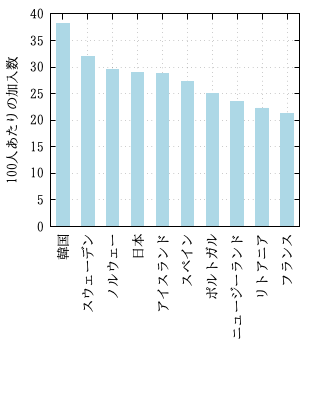
\includegraphics{fig11.png}
    \caption{光ファイバー回線の加入者人数（100人あたり）}
    \label{fig:光ファイバー回線の加入者人数}
\end{figure}

\section{デジタル競争力ランキング}

国際経営開発研究所（IMD）の査\cite{imd}によると,日本のデジタル競争力のランキングは表\ref{tbl:デジタル競争力ランキング}に示すように,
開査対象の64カ国中,総合で28位.技術分野で30位となっている.

\begin{table}[htbp]
    \centering
    \caption{デジタル競争力ランキング}
    \label{tbl:デジタル競争力ランキング}   

    \begin{tabular}{|c|c|c|}
        \hline
        国 & 総合 & 技術 \\
        \hline
        米国 & 1位 & 4位 \\
        \hline
        香港 & 2位 & 10位 \\
        \hline
        スウェーデン & 3位 & 8位 \\
        \hline
        デンマーク & 4位 & 2位 \\
        \hline
        シンガポール & 5位 & 3位 \\
        \hline
        韓国 & 12位 & 13位 \\
        \hline
        中国 & 15位 & 20位 \\
        \hline
        日本 & 28位 & 30位 \\
        \hline 
    
    \end{tabular}
\end{table}

\section{考察}
 \begin{itemize}
    \item 韓国の光ファイバーの普及率の高さは、各家庭にまで光ファイバーを引き込む政策が功を奏している
    と考えられ,その影響は韓国はが-sports大国と呼ばれる一因になっているであろう.

    また、デジタル競争力ランキングより、光ファイバーの普及率と、その国がデジタル力を持っているかどうかは、
    全く関係がないであろう.
    \item 光ファイバー普及率と,デジタル競争力の差異が大きいデンマークに注目すると,そもそもデンマークでは
    お金,移動,勉強など,生活のあらゆる面でデジタル化が進んでおり,パソコンやスマートフォンを使うことが当たり前になっている.
    光ファイバーの普及率の低さは,デンマークの立地条件が関係していると考えられ,デンマークは,国土の大部分が平地であり,都市部に人口が集中しているため,光ファイバーの設置数を抑えられているだろうと考える.
    
 \end{itemize}

% 本文(1
%  参考文献の参照: \cite{}
%  図番号の参照： \ref{}
% を使う
% 文献データベースのキーワードは oecd と imd
% になっている．

% 図の挿入
% \includegraphics{}
% を
% \begin{figure}[htbp]
% \end{figure}
% で囲み
% \caption{}
% で図のタイトルを入れる．
% \label{}
% を使って図番号が参照できるようにする
% また，
% \centering
% で図が中央に来るようにする

% ーーー
% 節見出し(2)

% 本文(2)

% 表の挿入
% \begin{tabular}
% \end{tabular}    
% による表の記述を 
% \begin{table}[htbp]
% \end{table}
% で囲み
% \caption{}
% で表のタイトルを入れる．
% \label{}
% を使って表番号が参照できるようにする
% また，
% \centering
% で表が中央に来るようにする

% ーーー
% 見出し(3)
% 考察
%
% \begin{itemize}
% \end{itemize}
% を使って箇条書きで記述する

% ここに参考文献が入る
%
\bibliographystyle{junsrt}
\bibliography{exercise.bib}

\end{document}